\documentclass[../main.tex]{subfiles}
\begin{document}

\section{Elevation}
Elevation will change how the player counts through their dice.

When the ball is about to enter a higher hex, the additional stacked hexes require additional dice to reach. The Dice used to determine the power of the stroke will also be used to determine if the ball can traverse the elevation. One dice  = 1 hex of elevation.

For example: A ball is on a hex facing a direction that is two hexes higher than its starting position. Still roll the dice as normal to determine spin, power, and wind resistance. One dice determines the spin. A minimum of two dice in the power category are required just to move up vertically, a total of three dice to traverse two hexes of elevation. 

\begin{figure}[h]
    \centering
    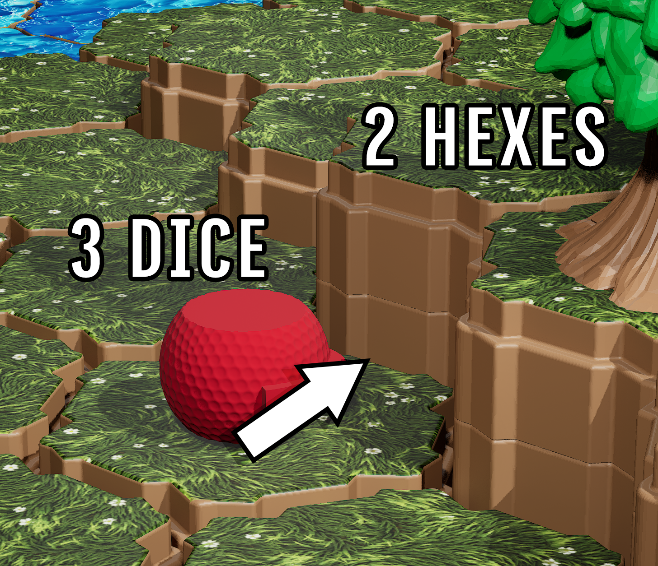
\includegraphics[width=1\linewidth]{chapters//Elevation.Putting.Winning/Source Golf HittingoverElevation.png}
\end{figure}

\section{Putting}

When a player lands their ball on the putting green without going into the hole, they will take one additional stroke. The ball will then be placed into the hole automatically, thus finishing their round. 

\section{Winning the Game}
Whomever has the least amount of strokes at the end of the round wins! Players can decide beforehand how many rounds they want to play and if they want to change the layout of the hole from round to round or change it every few rounds. 

\section{Playing Multiple Rounds}
Traditionally in golf, players play 18 holes in a session and keep their score tallied on a piece of paper to compare scores at the end. Players can do the same with Source Golf! Determine ahead of time how many holes everyone wants to play and keep the scores from each hole on a piece of paper, adding them up at the end to determine a winner! 

\begin{figure}[h]
    \centering
    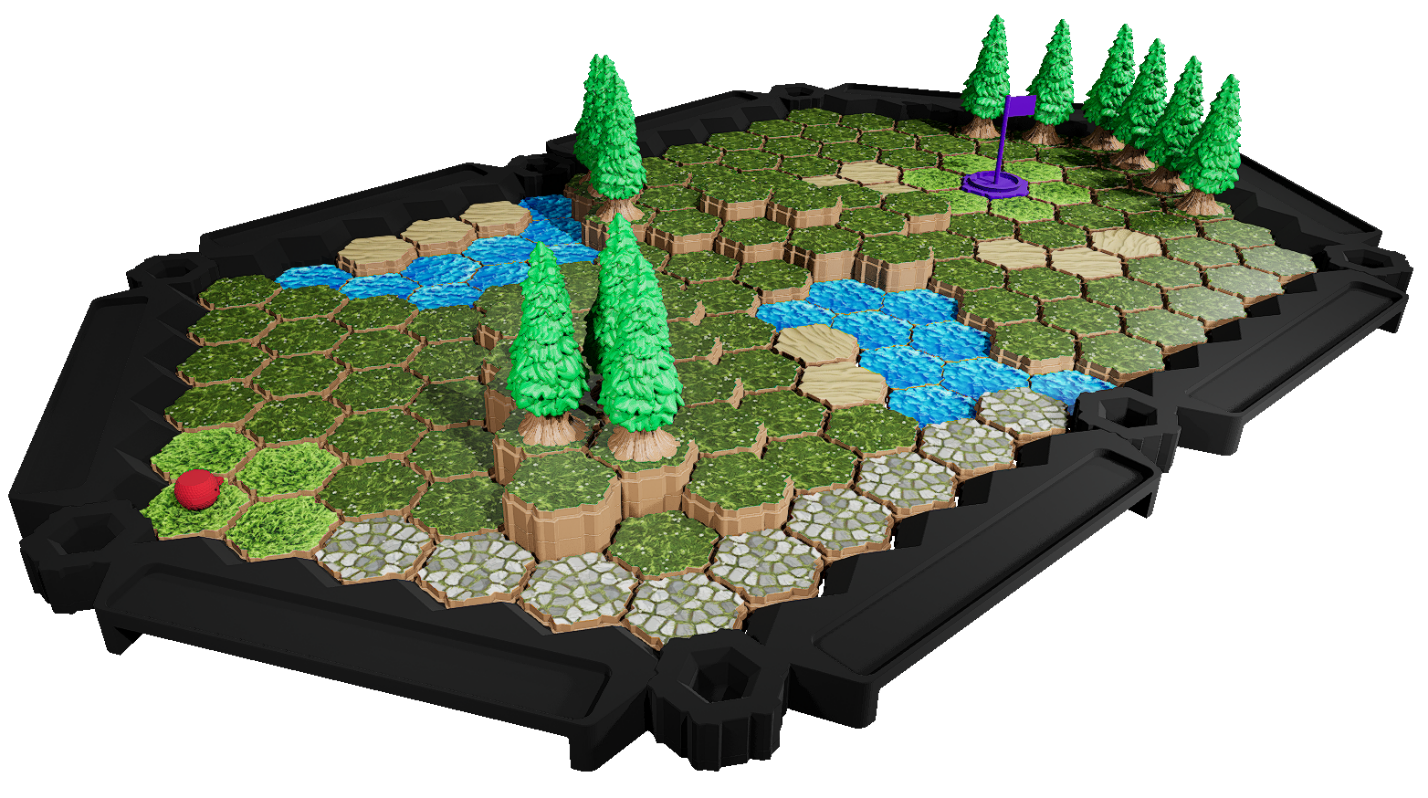
\includegraphics[width=1\linewidth]{chapters//Elevation.Putting.Winning/Source Golf full hole sideangle.png}   
\end{figure}

Have Fun! 

\end{document}